%%%%%% -*- Coding: utf-8-unix; Mode: latex

\documentclass[polish]{projectreport}
% \documentclass[english]{projectreport}

\usepackage[utf8]{inputenc}
\usepackage{url}
\usepackage{subfigure}
\usepackage{tabularx}
\usepackage{ragged2e}
\usepackage{booktabs}
\usepackage{multirow}
\usepackage{grffile}
\usepackage{float}
\usepackage{graphicx}
\usepackage{array}
\usepackage{diagbox}
\usepackage{tikz}
\usetikzlibrary{tikzmark, calc}


\usepackage[bookmarks=false]{hyperref}
\hypersetup{colorlinks,
  linkcolor=blue,
  citecolor=blue,
  urlcolor=blue}

\usepackage{indentfirst}
\usepackage{caption}
\usepackage{listings}
\usepackage[ruled,linesnumbered,lined]{algorithm2e}
\usepackage[svgnames]{xcolor}
\usepackage{inconsolata}
\usepackage{fancyhdr}

\usepackage{csquotes}
\DeclareQuoteStyle[quotes]{polish}
  {\quotedblbase}
  {\textquotedblright}
  [0.05em]
  {\quotesinglbase}
  {\fixligatures\textquoteright}
\DeclareQuoteAlias[quotes]{polish}{polish}

\usepackage[
style=numeric,
sorting=nyt,
isbn=false,
doi=true,
url=true,
backref=false,
backrefstyle=none,
maxnames=10,
giveninits=true,
abbreviate=true,
defernumbers=false,
backend=biber]{biblatex}
\addbibresource{bibliography.bib}

\lstset{
    %language=Python, %% PHP, C, Java, etc.
    basicstyle=\ttfamily\footnotesize,
    backgroundcolor=\color{gray!5},
    commentstyle=\it\color{Green},
    keywordstyle=\color{Red},
    stringstyle=\color{Blue},
    numberstyle=\tiny\color{Black},    
    % morekeywords={TestKeyword},
    % mathescape=true,
    escapeinside=`',
    frame=single, %shadowbox, 
    tabsize=2,
    rulecolor=\color{black!30},
    title=\lstname,
    breaklines=true,
    breakatwhitespace=true,
    framextopmargin=2pt,
    framexbottommargin=2pt,
    extendedchars=false,
    captionpos=b,
    abovecaptionskip=5pt,
    keepspaces=true,            
    numbers=left,                    
    numbersep=5pt,                  
    showspaces=false,                
    showstringspaces=false,
    showtabs=false,
    tabsize=2
}

\SetAlgorithmName{\LangAlgorithm}{\LangAlgorithmRef}{\LangListOfAlgorithms}

\renewcommand{\lstlistingname}{\LangListing}
\renewcommand\lstlistlistingname{\LangListOfListings}

\newcolumntype{Y}{>{\small\centering\arraybackslash}X}
%\newcolumntype{b}{>{\hsize=1.6\hsize}Y}
%\newcolumntype{m}{>{\hsize=.6\hsize}Y}
%\newcolumntype{s}{>{\hsize=.4\hsize}Y}

\captionsetup[figure]{skip=5pt,position=bottom}
\captionsetup[table]{skip=5pt,position=top}



%%%%%%%%%%%%%%%%%%%%%%%%%%%%%%%%%%%%%%%%%%%%%%%%%%%%%%%%%%%%%%%%%%%%%%%%%%%%%%%
\author{Piotr Sielchanowicz \\ Marcin Walendzik}

\title{\textbf{Symulacja ruchu drogowego na Południowej Obwodnicy Warszawy (POW) na odcinku od węzła "Puławska" (bez węzła) do węzła "Czerniakowska" (bez węzła) na podstawie prognoz ruchu dla roku 2035}}

\raggedbottom

%%%%%%%%%%%%%%%%%%%%%%%%%%%%%%%%%%%%%%%%%%%%%%%%%%%%%%%%%%%%%%%%%%%%%%%%%%%%%%%
\begin{document}

\maketitle

\thispagestyle{empty}


%%%%%%%%%%%%%%%%%%%%%%%%%%%%%%%%%%%%%%%%%%%%%%%%%%%%%%%%%%%%%%%%%%%%%%%%%%%%%%% 

\vspace{6cm}

\begin{abstract}
W niniejszym artykule przedstawiono analizę warunków ruchu na wybranym odcinku Południowej Obwodnicy Warszawy (S2). Wykorzystując środowisko mikrosymulacyjne SUMO Eclipse, zbadano wpływ pięciu różnych scenariuszy natężenia ruchu (od 50\% do 140\% ruchu bazowego) na globalną efektywność sieci. Wyniki eksperymentów wykazały, że sieć osiąga stan krytyczny przy skali ruchu 0.75, gdzie średni czas oczekiwania pojazdów wzrasta o kilkaset procent, a na pasach włączania zaczynają generować się permanentne zatory drogowe.
\end{abstract}

\vspace{2cm}
\noindent \textbf{Keywords:} mikrosymulacja ruchu, SUMO Eclipse, przepustowość, węzły drogowe, S2, droga ekspresowa, obwodnica Warszawy.

%%%%%%%%%%%%%%%%%%%%%%%%%%%%%%%%%%%%%%%%%%%%%%%%%%%%%%%%%%%%%%%%%%%%%%%%%%%%%%% 

\newpage

\section{Wstęp i przegląd literatury tematycznej}
\label{sec:introduction}

Niniejsza praca jest dokumentacją projektową skupiającą się na tematyce symulacji ruchu drogowego. Realizacja projektu wynika z założeń przedmiotu Symulacji i modelowania systemów, w ramach, którego należało przeprowadzić symulację systemu z określonej w ramach zajęć tematyki. Za kategorię podmiotu rozważań, autorzy wybrali symulację z zakresu ruchu drogowego. \\

Symulacja drogowa jest istotną procedurą w zakresie tworzenia nowych inwestycji. Dzięki niej, można w odpowiedni sposób wyznaczyć kierunek tworzenia infrastruktury, mając na celu:
\begin{itemize}
    \item redukcję ruchu,
    \item wskazanie kluczowych dla projektu rozwiązań poprawiających infrastrukturę,
    \item minimalizację negatywnego wpływu na środowisko,
    \item weryfikację przepustowości infrastruktury,
    \item ograniczenie ryzyka inwestycyjnego, dzięki przetestowaniu rozwiązania w formie cyfrowej.
\end{itemize}


%%%%%%%%%%%%%%%%%%%%%%%%%%%%%%%%%%%%%%%%%%%%%%%%%%%%%%%%%%%%%%%%%%%%%%%%%%%%%%% 
\subsection{Tematyka oraz cel symulacji}
\label{sec:topic}

Przedmiotem rozważań oraz poddania planowanej symulacji jest inwestycja drogowa znajdująca się na terenie miasta stołecznego Warszawa - fragment \textbf{Południowej Obwodnicy Warszawy (POW) od węzła "Puławska" (bez węzła) do węzła "Czerniakowska" (bez węzła)}. Projekt ten jest już zakończony w całości od roku 2021. Pomimo, że aktualnie realizowanych jest wiele inwestycji z zakresu rozwoju drogowego kraju, autorzy postanowili wybrać tą inwestycję, ze względu na względnie łatwo dostępną analizę ruchu po opisywanej infrastrukturze \cite{pow_analiza}. W innych przypadkach, szczególnie w przypadku nadzorowania przez GDDKiA, dokumentacja jest niedostępna internetowo, a w przypadku skierowania prośby o wydanie analiz należy uwzględnić czas odpowiedzi strony administracyjnej. Autorom najbardziej zależało na danych, które były dostępne natychmiast i w prosty sposób. Analiza budowy wspominanego odcinka POW posiada bardzo szczegółową dokumentację, w której znaleźć można komplet informacji potrzebnych do przeprowadzenia symulacji mikroskopowej.  \\

\noindent Analiza odcinka będącego tematem niniejszej pracy składa się z dwóch części:
\begin{itemize}
    \item \textbf{analizy prognoz ruchu},
    \item \textbf{przeprowadzenie symulacji na podstawie danych i ich analiza}.
\end{itemize}

Autorzy zdecydowali, że symulacji będzie podlegać jedynie część infrastruktury opisanej w dokumencie. Przytaczana analiza skupia się na opisuje ruch na POW na fragmencie między węzłami "Puławska" i "Lubelska" z wyłączeniem tych węzłów, natomiast planowana symulacja ma się skupić na ruchu między węzłami "Puławska" i "Czerniakowska", podobnie jak w opracowaniu, nie skupiając się na węzłach brzegowych. Decyzja ta jest podyktowana danymi dostępnymi w analizie. Pomimo, że prognozy ruchu na rok 2035, które są podstawą dla symulacji ruchu drogowego obejmują większą część infrastruktury, to czytelnik nie znajdzie tam danych dotyczących dokładnego ruchu z danego punktu wjazdowego do konkretenego wyjazdowego. Podane są dane jedynie dla ogółu pojazdów, które przejadą przez jezdnię 
% przypis
(przez jezdnię rozumie się pasy ruchu w jednym kierunku dla, których w dokumentacji wskazana jest jedna liczba pojazdów wjeżdżających / wyjeżdżających). Przeprowadzenie symulacji natomiast, wymaga podania konkretnej trasy i liczebności agentów z punktu A do punktu B. Wymaga to obliczenia z posiadanych danych tras o pewnej liczbie aut, a także wyaproksymowanie liczby aut na trasach, na których takiej pewnej liczby nie da się otrzymać, z zachowaniem względnie poprawnych liczb względem oryginalnych danych. Liczba takich aproksymacji przy całej inwestycji od węzła "Puławska" do węzła "Lubelska" byłaby dużo większa, co znacząco obniżyło by tempo prac, jak i zwiększyło trudność przygotowania symulacji. \\

Wśród wspomnianych powyżej analiz ruchu, autorzy tychże określili przewidywany ruch samochodowy na rok 2035. Prognozy te zawierają dane dotyczące średniej liczby pojazdów w ramach każdej jezdni wejściowej oraz wyjściowej. Informacje te zostały przedstawione graficznie, osobno dla każdego węzła. 

\begin{figure}[htbp]
    \centering
    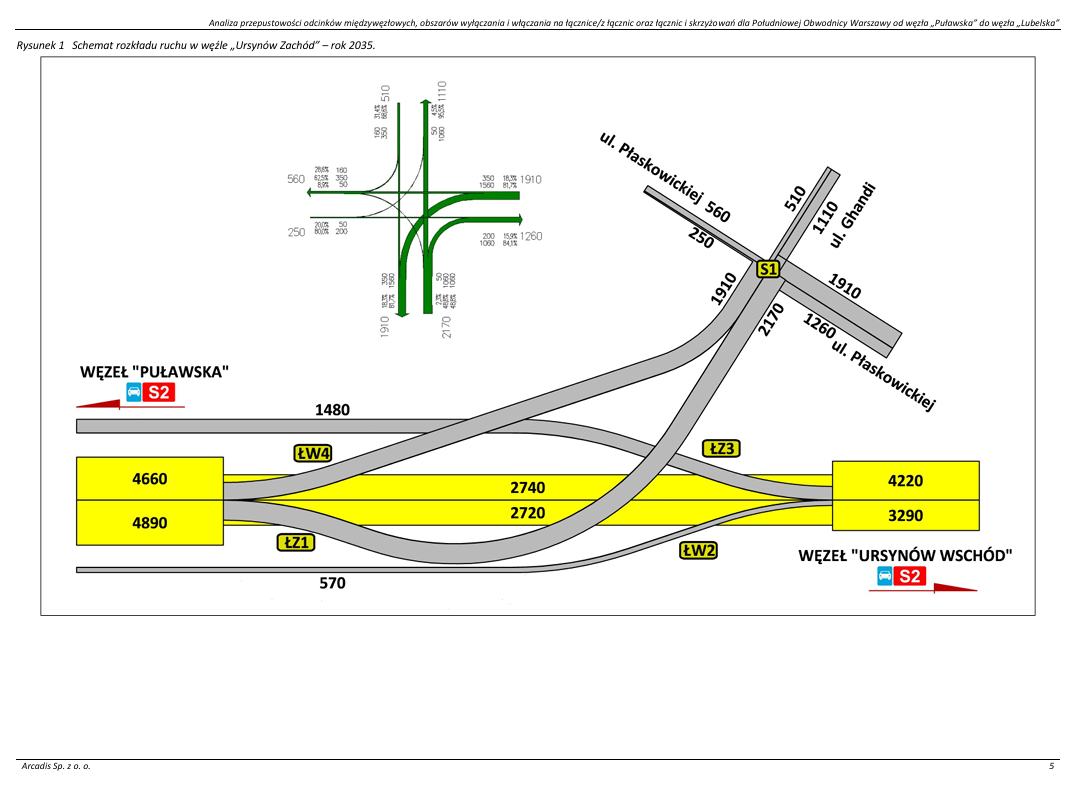
\includegraphics[width=1.0\linewidth]{img/road_traffic_on_Ursynow_Zachod.png}
    \caption{Schemat rozkładu ruchu na jednym z analizowanych węzłów "Ursynów Zachód"}
    \label{fig:placeholder}
\end{figure}

Analizy posiadają również ocenę wydolności odcinków, jak i węzłów przy spodziewanym poziomie ruchu. Według prognoz, część odcinków na rok 2035, będzie posiadała ograniczoną płynność ruchu, szczególnie w godzinach szczytu. Niniejsza praca, ma na celu próbę odtworzenia w środowisku komputerowym i ocenę trafności przewidywanych warunków ruchu. Dodatkowo, ze względu na istotność tej infrastruktury autorzy planują sprawdzić warunki, dla których ruch na POW stanie się na tyle duży, że dojdzie do zatłoczenia na drodze i przekroczenia dopuszczalnej przepustowości drogi w warunkach rzeczywistych. \\

Na stronie inwestycji dostępne prócz analiz i prognoz ruchu są również dane techniczne dotyczące projektowanej drogi \cite{siskom_strona}. Znajdują się tam pliki graficzne przedstawiające stałą organizację ruchu, w tym znaki drogowe, ilość pasów danego odcinka, ich długość, szerokość.

%%%%%%%%%%%%%%%%%%%%%%%%%%%%%%%%%%%%%%%%%%%%%%%%%%%%%%%%%%%%%%%%%%%%%%%%%%%%%%%

\subsection{Wybór narzędzia do przeprowadzenia symulacji}
\label{sec:simulation-tools}

Pierwszym krokiem koniecznym do przeprowadzenia symulacji był wybór środowiska do symulacji. W tym celu autorzy skorzystali z badań dostępnych w Internecie z rozważanej tematyki, w której analizowano przynajmniej kilka różnych oprogramowań. \\

W publikacji z roku 2010 autorstwa Michała Maciejewskiego na przykładzie skrzyżowania miejskiego z Poznania zestawione zostały trzy programy: TRANSIMS (TRansportation ANalysis and SIMulation System), SUMO (Simulation of Urban MObility) oraz PVT Vissim \cite{sim_comparison}. Przy ich pomocy przeprowadzono symulacje dla ruchu na wskazanym skrzyżowaniu i dokonano ich porównania, z którego wnioski zostały zaprezentowane w tabeli.

\begin{figure}[H]
    \centering
    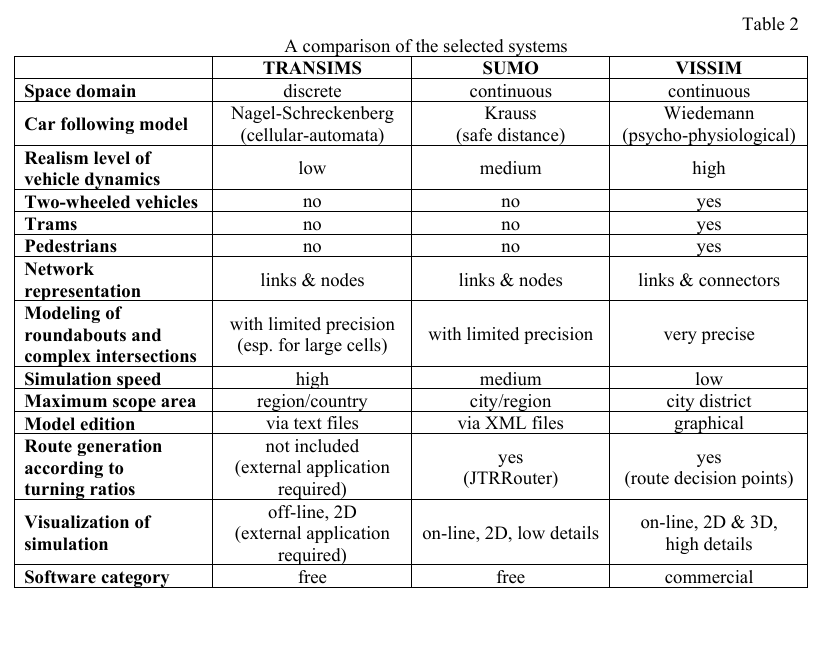
\includegraphics[width=0.75\linewidth]{img/simmulators_comparison.png}
    \caption{Zestawienie cech i własności analizowanych symulatorów}
    \label{fig:placeholder}
\end{figure}

Z zestawienia oraz opisów przeprowadzonych symulacji, można wyciągnąć wnioski, iż najrozsądniejszym wyborem do przeprowadzenia symulacji POW będzie SUMO. Główymi zaletami tego programu są fakt, iż jest darmowy, a także jest stosowany z powodzeniem do symulacji ruchu miejskiego. Z przytaczanego badania można zauważyć, że jest on bardziej precyzyjny, niż inny darmowy program TRANSIMS, a dodatkowo korzysta z ciągłego modelu śledzenia (model Krauss). W analizie podkreślono, że najbardziej precyzyjnym narzędziem z naszej tematyki jest Vissim, jednak program ten nie jest dostępny bezpłatnie. Ma on sporą przewagę nad innymi programami na polu dokładniejszego modelowania sieci dróg, jednak jest on dostępny odpłatnie. \\

Przed wyborem narzędzia została także przeprowadzona dogłębna analiza innych możliwości, jednakże nie posiadały one potrzebnych cech lub wymagałyby nadmiarowej pracy, która nie przekładałaby się na efekt końcowy. Część z nich nie udostępniała również możliwości symulacji na danych dostępnych z prognoz. \\

\newpage

%%%%%%%%%%%%%%%%%%%%%%%%%%%%%%%%%%%%%%%%%%%%%%%%%%%%%%%%%%%%%%%%%%%%%%%%%%%%%%%
\noindent \textbf{Pozostałe narzędzia:}
% \label{sec:lists}

\begin{itemize}
    \item AnyLogic,
    \item Aimsun,
    \item SIDRA Intersection,
    \item AutoTURN,
    \item Pygame,
    \item Godot,
    \item Cities Skylines 2,
    \item Transport Fever 2,
    \item Mini Motorways.
\end{itemize}

Po analizach autorzy do symulacji rozważanego projektu wybrali \textbf{SUMO}, który zapewnia rozsądny poziom szczegółowości oraz darmowy dostęp, co w ocenie autorów jest rozsądnym kompromisem z pomiędzy pozostałych narzędzi \cite{sumo_page}. 

%%%%%%%%%%%%%%%%%%%%%%%%%%%%%%%%%%%%%%%%%%%%%%%%%%%%%%%%%%%%%%%%%%%%%%%%%%%%%%%
% \subsection{Inne symulacje}
% %Inne symulacje / prace naukowe odnośnie ruchu drogowego
% Do rzetelnego wykonania projektu niezbędna była także analiza podobnych symulacji realizowanych przez inne jednostyki naukowe oraz prywatne.

% \begin{itemize}
% \item \href{https://traffic-simulation.de/}{traffic-simulation.de}
% \item \href{https://www.anylogic.com/road-traffic/}{anylogic trafic simulator}
% \item \href{https://github.com/cityflow-project/CityFlow/}{CityFlow}
% \item \href{https://github.com/TheDuckCow/godot-road-generator}{godot-road-generator}
% \end{itemize}
%%%%%%%%%%%%%%%%%%%%%%%%%%%%%%%%%%%%%%%%%%%%%%%%%%%%%%%%%%%%%%%%%%%%%%%%%%%%%%%

\newpage

\section{Model symulacyjny oraz algorytmy i biblioteki}
\label{sec:solution}

Z wymienionych i analizowanych dotychczas środowisk symulacyjnych autorzy wybrali program Eclipse SUMO (Simulation of Urban MObility). Jest on symulatorem specjalnie przystosowanym do symulacji ruchu samochodowego - umożliwia proste emulowanie natężeń ruchu na drogach oraz testy przepustowości zaprojektowanych połączeń. 

\subsection{Przygotowanie modelu}

Na stworzenie symulacji programu SUMO składa się stworzenie mapy infrastruktury drogowej (pliki z rozszerzeniem \texttt{.net.xml}) oraz konfiguracja tras agentów (pliki z rozszerzeniem \texttt{.rou.xml}). Przy użyciu kilku dodatkowych konfiguracji można przy pomocy sumo gui, bądź komendy w wierszu poleceń stworzyć na ich podstawie plik symulacyjny (\texttt{.sumocfg}). \\

\subsubsection{Stworzenie mapy}
% \noindent \textbf{Stworzenie mapy} \\

Stworzenie mapy odbyło się za pomocą narzędzia wbudowanego w SUMO - osmWebWizard. Jest on zrealizowany jako skrypt języka python, który korzysta z internetowej usługi OSM (\textit{Open Street Map}), która udostępnia mapę infrastruktury drogowej. Narzędzie osmWebWizard pozwala poprzez interfejs graficzny na zaznaczenie interesującego użytkownika obszaru i pobranie określonych przez niego struktur. Dodatkowo, istnieje również opcja, aby bezpośrednio z tego programu dodać prostą konfigurację pojazdów. \\

\begin{figure}[H]
    \centering
    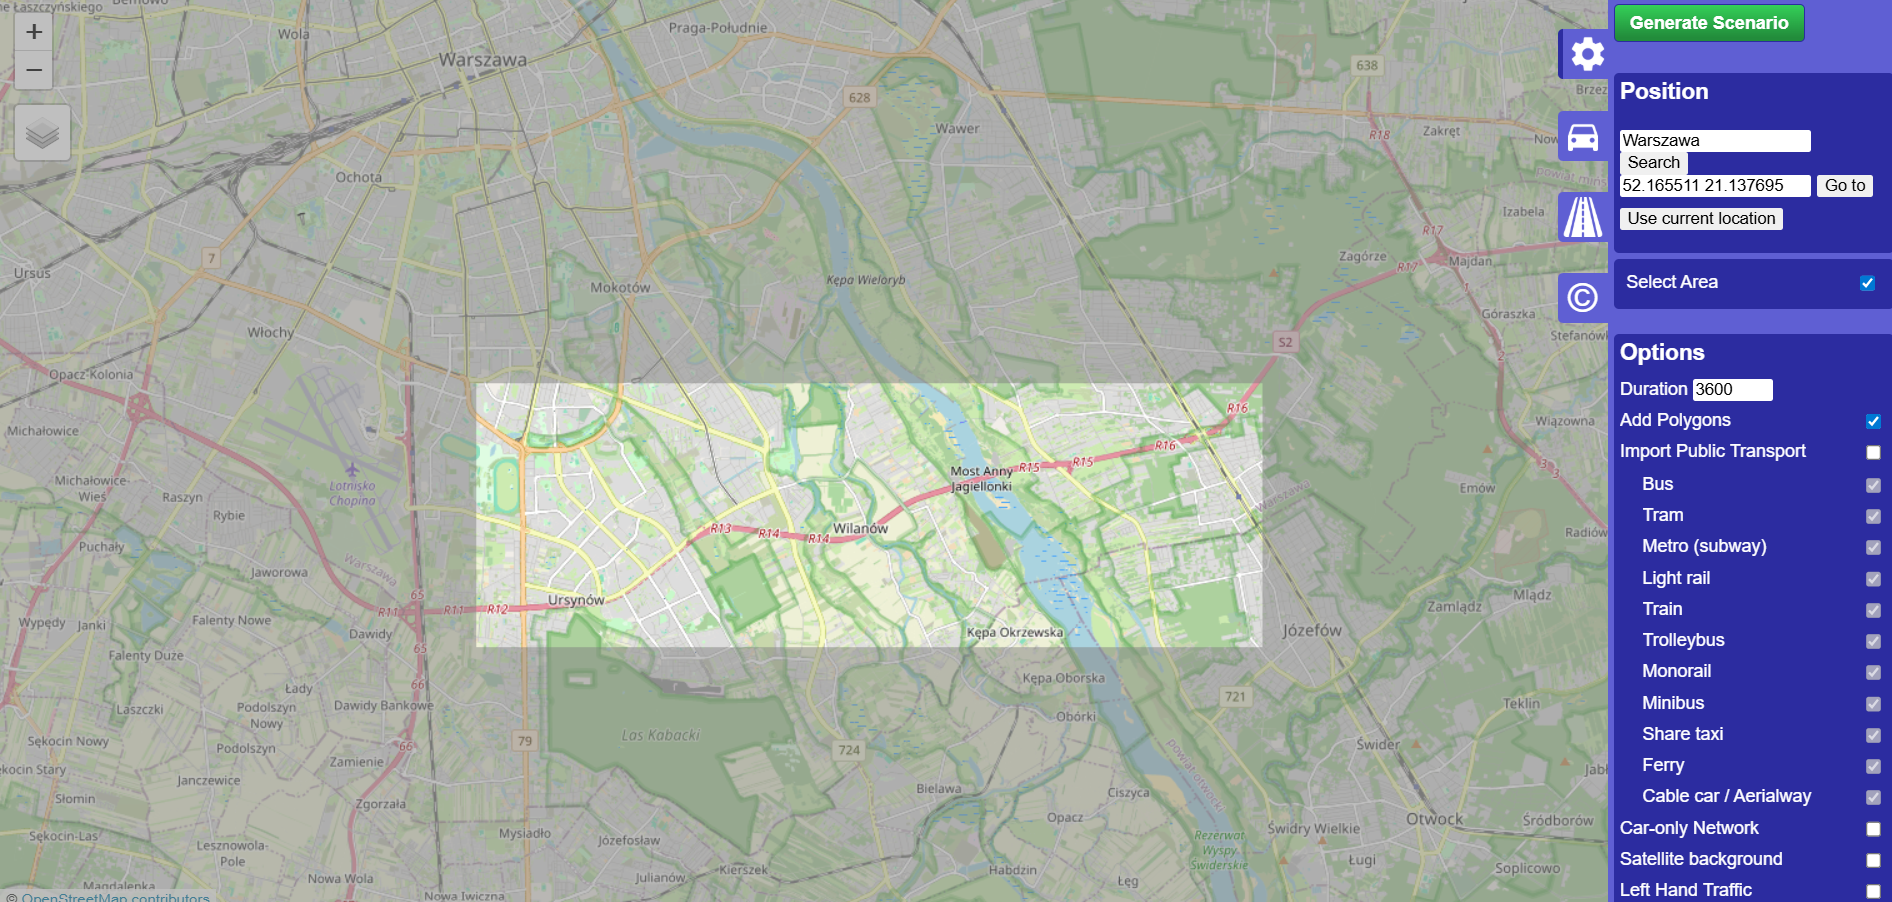
\includegraphics[width=0.9\linewidth]{img/map_creation.png}
    \caption{Eksportowanie mapy przy użyciu narzędzia osmWebWizard}
    \label{fig:map_creation}
\end{figure}

Przeprowadzenie tego kroku zajęło sporo czasu ze względu na problem z komunikacją z api obsługującego pobieranie mapy. W najnowszej wersji dostępnej na stronie oprogramowania 1.26.0 nie było możliwe uruchomienie i pobranie z powodzeniem plików. Rozwiązaniem okazało się uruchomienie narzędzia na buildzie deweloperskim. \\

\begin{figure}[H]
    \centering
    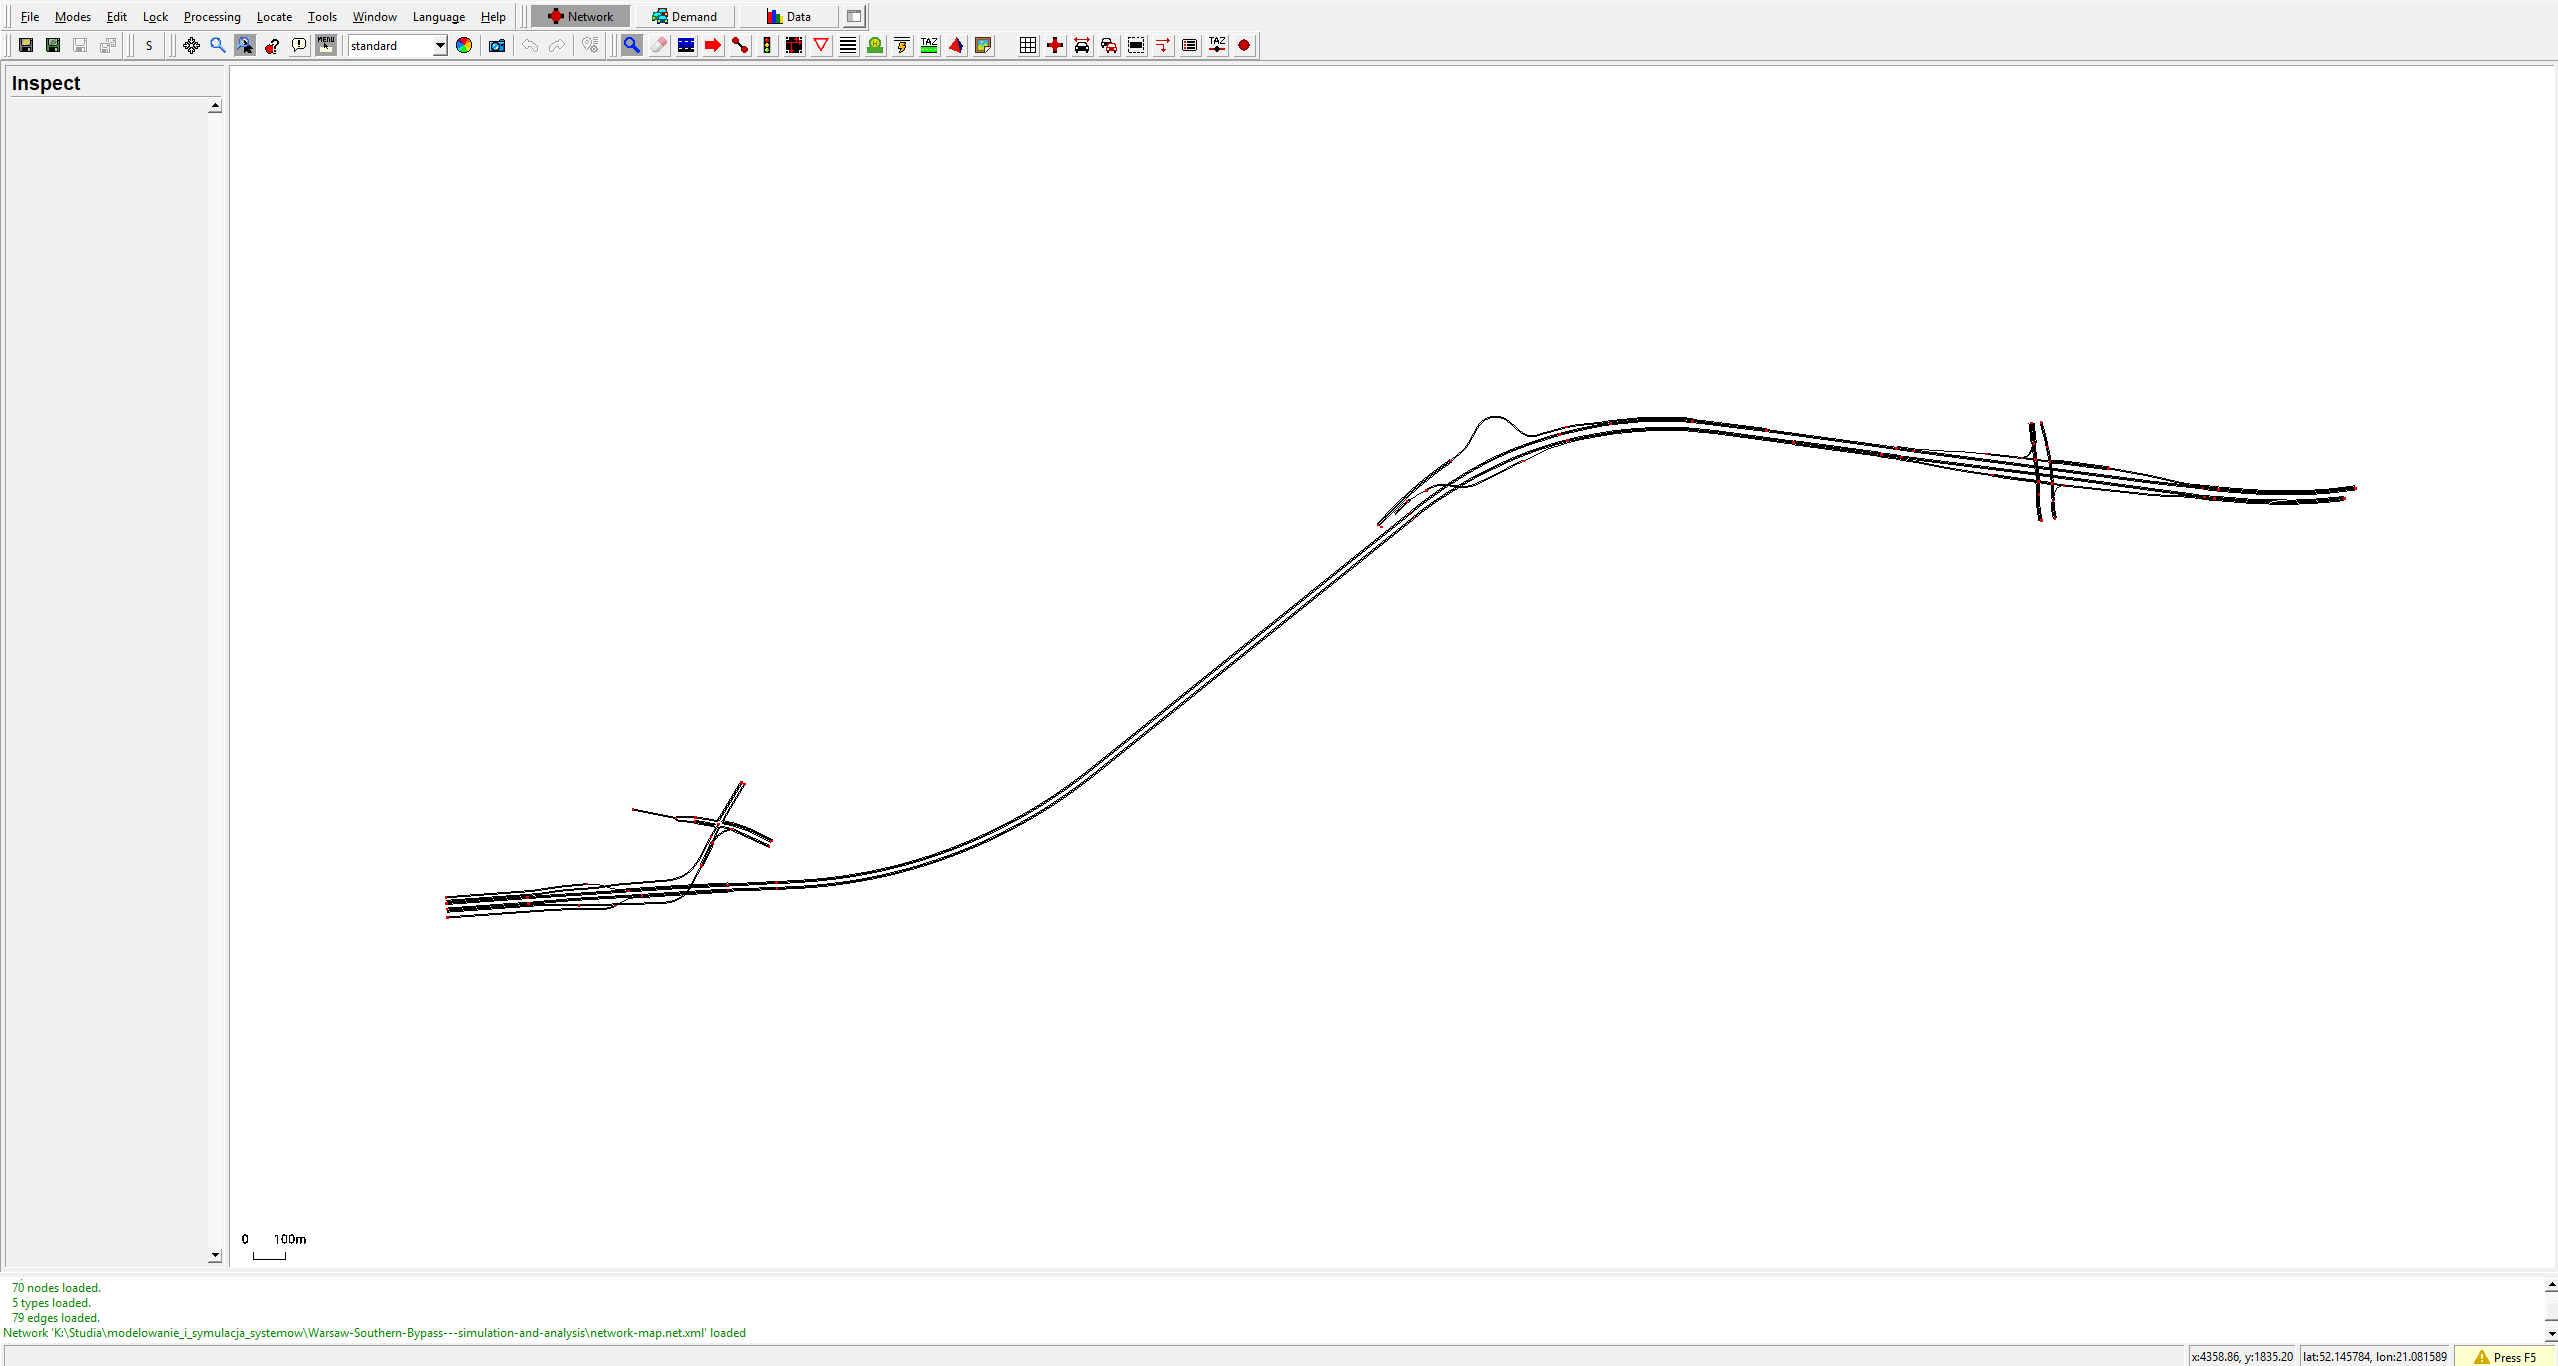
\includegraphics[width=0.9\linewidth]{img/network_cut.png}
    \caption{Mapa symulacji}
    \label{fig:network}
\end{figure}

Po pobraniu mapy, w narzędziu netedit usunięte zostały boczne ulice i zostawiono jedynie istotną dla symulacji część infrastruktury. \\

\subsubsection{Przygotowanie danych tras ruchu agentów}

Tak jak wspomniano wcześniej, w celu przeprowadzenia symulacji autorzy potrzebowali konkretnej liczby pojazdów poruszających się z konkretnej jezdni wjazdowej do konkretnej jezdni wyjazdowej. W tym celu, z danych dostępnych z grafik należało obliczyć pewne liczby związane z przepływem przy kilku założeniach:

\begin{itemize}
    \item Nie uwzględniamy w liczbach ruchu aut zawracających - np. auto wjeżdżające na od strony węzła "Puławska", nie pojedzie z powrotem w kierunku tego węzła.
    \item Nie uwzględniamy w liczbach ruchu pojazdów tras, które wymagały by choć częściowego zawrócenia, np. auto wjeżdżając od strony łącznika wjazdowego S2 na węźle "Ursynów Zachód", nie pojedzie do ul. Gandhi, ani ul. Płaskowickiej, ponieważ wymagałoby to zawrócenia na węźle "Przyczółkowska".
    \item Wszystkie pozostałe trasy są efektywnie najkrótsze jak to możliwe.
\end{itemize}

Założenia te wynikały częściowo ze względu na to, że droga, którą obejmuje inwestycja nie jest jedyną w rejonie. Mocno rozbudowana infrastruktura miasta stołecznego Warszawa w tamtej okolicy sprawia, że większość wykluczonych tras jest nieefektywna, jeśli by jechać w danym kierunku przy użyciu drogi obwodnicy. Warto zwrócić uwagę, że część obwodnicy jest poprowadzona tunelem bądź estakadą, co sprawia, że drogi lokalne są poprowadzone nad lub pod nią obsługując ruch lokalny. Dopiero dalszy ruch, w większości tranzytowy, jest dużo efektywniejszy przy użyciu obwodnicy, czyli przykładowo dla trasy od węzła "Puławska" do węzła "Lubelska". \\

\newpage

\begin{table}[htbp]
\centering
\caption{Zestawienie łącznej liczby aut wjeżdżających na daną jezdnię w symulacji, danych oryginalnych oraz ich różnicy. W zestawieniu dodano również ID, które zostały zastosowane w  pliku sieci .net.xml do konfiguracji tras ruchu}
\label{tab:zestawienie_danych}
\renewcommand{\arraystretch}{1.2}
\begin{tabular}{l|c|r|r|r}
\hline
\textbf{Nazwa węzła} & \textbf{ID} & \textbf{\shortstack{Liczba aut\\(symulacja)}} & \textbf{\shortstack{Dane\\oryginalne}} & \textbf{Różnica} \\ \hline
Ursynów Zach. wjazd             & s2  & 4900 & 4890 & -10 \\
Ursynów Zach. wyjazd            & s1  & 4710 & 4660 & -50 \\
Ursynów Zach. ŁW2               & w3  & 570  & 570  & 0   \\
Ursynów Zach. ŁZ3               & w4  & 1480 & 1480 & 0   \\
ul. Płaskowickiej Zach. wyjazd  & p1  & 560  & 560  & 0   \\
ul. Płaskowickiej Zach. wjazd   & p2  & 250  & 250  & 0   \\
ul. Płaskowickiej Wsch. wyjazd  & p3  & 1260 & 1260 & 0   \\
ul. Płaskowickiej Wsch. wjazd   & p4  & 1910 & 1910 & 0   \\
ul. Gandhi wjazd                & g1  & 510  & 510  & 0   \\
ul. Gandhi wyjazd               & g2  & 1110 & 1110 & 0   \\
Ursynów Wsch. ŁW1               & l2  & 1070 & 1070 & 0   \\
Ursynów Wsch. ŁZ2               & l1  & 1650 & 1720 & +70 \\
ul. Przyczółkowska Płn. wyjazd  & pr1 & 2840 & 2840 & 0   \\
ul. Przyczółkowska Płn. wjazd   & pr2 & 2240 & 2250 & +10 \\
ul. Przyczółkowska Płd. wyjazd  & pr3 & 890  & 890  & 0   \\
ul. Przyczółkowska Płn. wjazd   & pr4 & 1790 & 1800 & +10 \\
Przyczółkowska Wsch. wyjazd     & e1  & 6070 & 6060 & -10 \\
Przyczółkowska Wsch. wjazd      & e2  & 4810 & 4810 & 0   \\ \hline
\end{tabular}
\end{table}

Otrzymane w powyższej tabeli (Tabela~\ref{tab:zestawienie_danych}) wyniki są pochodną sumarycznej ilości aut wjeżdżających lub zjeżdżających na danych jezdniach po zastosowaniu obliczonych przez autorów liczebności tras (Tabela~\ref{tab:macierz}). Różnica między danymi oryginalnymi, a tymi, które są wynikiem konfiguracji tras autorów są w ich opinii dość podobne i zadawalające, na tyle, żeby przyjąć je jako dane, o które można oprzeć symulację nieodbiegając od prognoz. Różnice są na tyle niewielkie, że nie powinny zakłócić ostatecznego obrazu i wniosków eksperymentu. \\

Poniżej zestawiona jest macierz ruchu od - do, której dane zostaną zastosowane do dostosowania konfiguracji tras ruchów w symulatorze. \\

\newcommand{\rotpion}[1]{\multicolumn{1}{c}{\rotatebox{90}{\rule{3mm}{0pt}\textbf{#1}\rule{2mm}{0pt}}}}

\begin{table}[H]
\centering
\caption{Macierz ruchu}
\label{tab:macierz}

\setlength{\tabcolsep}{6pt}
\renewcommand{\arraystretch}{1.2}

\begin{tabular}{l|ccccccccc}
\hline

\multicolumn{1}{c|}{%
\begin{tikzpicture}
\node[
    minimum width=3.5cm,
    minimum height=5.5cm,
    inner sep=0pt
] (c) {};

\draw[thick] (c.north west) -- (c.south east);

\node[anchor=north east,font=\bfseries]
at ([xshift=-2mm,yshift=-2mm]c.north east) {Do};

\node[anchor=south west,font=\bfseries]
at ([xshift=2mm,yshift=2mm]c.south west) {Skąd};
\end{tikzpicture}
}
&
\rotpion{Ursynów Zach. wyjazd}
&
\rotpion{Ursynów Zach. ŁZ3}
&
\rotpion{ul. Płaskowickiej Zach. wyjazd}
&
\rotpion{ul. Płaskowickiej Wsch. wyjazd}
&
\rotpion{ul. Gandhi wyjazd}
&
\rotpion{Ursynów Wsch. ŁZ2}
&
\rotpion{ul. Przyczółkowska Płn. wyjazd}
&
\rotpion{ul. Przyczółkowska Płd. wyjazd}
&
\rotpion{Przyczółkowska Wsch. wyjazd}
\\ \hline

\textbf{Ursynów Zach. wjazd}           & -    & -    & 50   & 1060 & 1060 & -    & 230  & 100 & 2400 \\
\textbf{Ursynów Zach. ŁW2}             & -    & -    & -    & -    & -    & -    & 30   & 10  & 530  \\
\textbf{ul. Płaskowickiej Zach. wjazd} & -    & -    & -    & 200  & 50   & -    & -    & -   & -    \\
\textbf{ul. Płaskowickiej Wsch. wjazd} & 1560 & -    & 350  & -    & -    & -    & -    & -   & -    \\
\textbf{ul. Gandhi wjazd}              & 350  & -    & 160  & -    & -    & -    & -    & -   & -    \\
\textbf{Ursynów Wsch. ŁW1}             & -    & -    & -    & -    & -    & -    & 50   & 20  & 1000 \\
\textbf{ul. Przyczółkowska Płn. wjazd} & 440  & 140  & -    & -    & -    & 160  & -    & 710 & 790  \\
\textbf{ul. Przyczółkowska Płd. wjazd} & 260  & 80   & -    & -    & -    & 90   & 1270 & -   & 90   \\
\textbf{Przyczółkowska Wsch. wjazd}    & 2100 & 1260 & -    & -    & -    & 1400 & 1260 & 50  & -    \\ \hline
\end{tabular}
\end{table}

\subsection{Stworzenie tras ruchów agentów}

Posiadając już gotowe do zastosowania dane przystąpiono do stworzenia pliku \texttt{.flows.xml}. W pliku tym zostały naniesione potoki ruchu wynikające z macierzy (Tabela~\ref{tab:macierz}). \\

\begin{lstlisting}[language=XML, caption={Fragment definicji potoków ruchu w pliku flows.flows.xml}, label={lst:xml-flows}]
<routes xmlns:xsi="http://www.w3.org/2001/XMLSchema-instance"
        xsi:noNamespaceSchemaLocation="http://sumo.dlr.de/xsd/routes_file.xsd">
    
    <!-- from: s2 -->
    <flow id="f_s2_to_e2" from="s2" to="e2" begin="0" end="3600" number="2400"/>
    <flow id="f_s2_to_g2" from="s2" to="g2" begin="0" end="3600" number="1060"/>
    <flow id="f_s2_to_p1" from="s2" to="p1" begin="0" end="3600" number="50"/>
    ...
</routes>
\end{lstlisting}

Na podstawie tych potoków oraz pliku sieci (\texttt{.net.xml}) za pomocą narzędzia SUMO \texttt{duarouter} użytkownik jest w stanie wygenerować plik \texttt{.rou.xml}, który jest finalnym plikiem potrzebnym do uruchomienia symulacji. Dzięki wspomnianemu narzędziu, w pliku \texttt{routes.rou.xml} otrzymujemy pełną listę tras dla wszystkich agentów podczas trwania całej symulacji.

Krok ten został wykonany przy pomocy konsolowej komendy:

\texttt{duarouter -n network-map.net.xml -r flows.flows.xml -o routes.rou.xml}

%%%%%%%%%%%%%%%%%%%%%%%%%%%%%%%%%%%%%%%%%%%%%%%%%%%%%%%%%%%%%%%%%%%%%%%%%%%%%%%
\section{Przeprowadzenie symulacji}

Uruchomienie symulacji w programie Eclipse SUMO wymaga posiadania przynajmniej dwóch plików - pliku sieci (\texttt{.net.xml}) oraz pliku tras agentów (\texttt{.rou.xml}). Obydwa te pliki zostały wygenerowane podczas poprzednich kroków. Ostatnim krokiem jest uruchomienie symulacji. \\

SUMO umożliwia przeprowadzenie symulacji na dwa sposoby. Pierwszym jest przeprowadzenie tego w wersji konsolowej. Wystarczu do tego zwykłe polecenie w wierszu poleceń: \\

\noindent\texttt{sumo -n network.net.xml -r routes.rou.xml} \\

Drugim sposobem jest przeprowadzenie tego w interfejsie graficznym SUMO, gdzie użytkownik jest w stanie zobaczyć jak w aktualnej sekundzie symulacji wygląda ruch i wizualnie obserwować zachowanie aut na drodze. Służy do tego komenda: \\

\noindent\texttt{sumo-gui -n network.net.xml -r routes.rou.xml} \\

Istnieje również opcja zapisania konfiguracji symulacji, dzięki czemu nie istnieje potrzeba ciągłego podawania plików sieci oraz tras przy wywołaniu symulatora:

\noindent\texttt{sumo-gui -n network.net.xml -r routes.rou.xml --save-configuration simulation.sumocfg} \\

\begin{figure}[H]
    \centering
    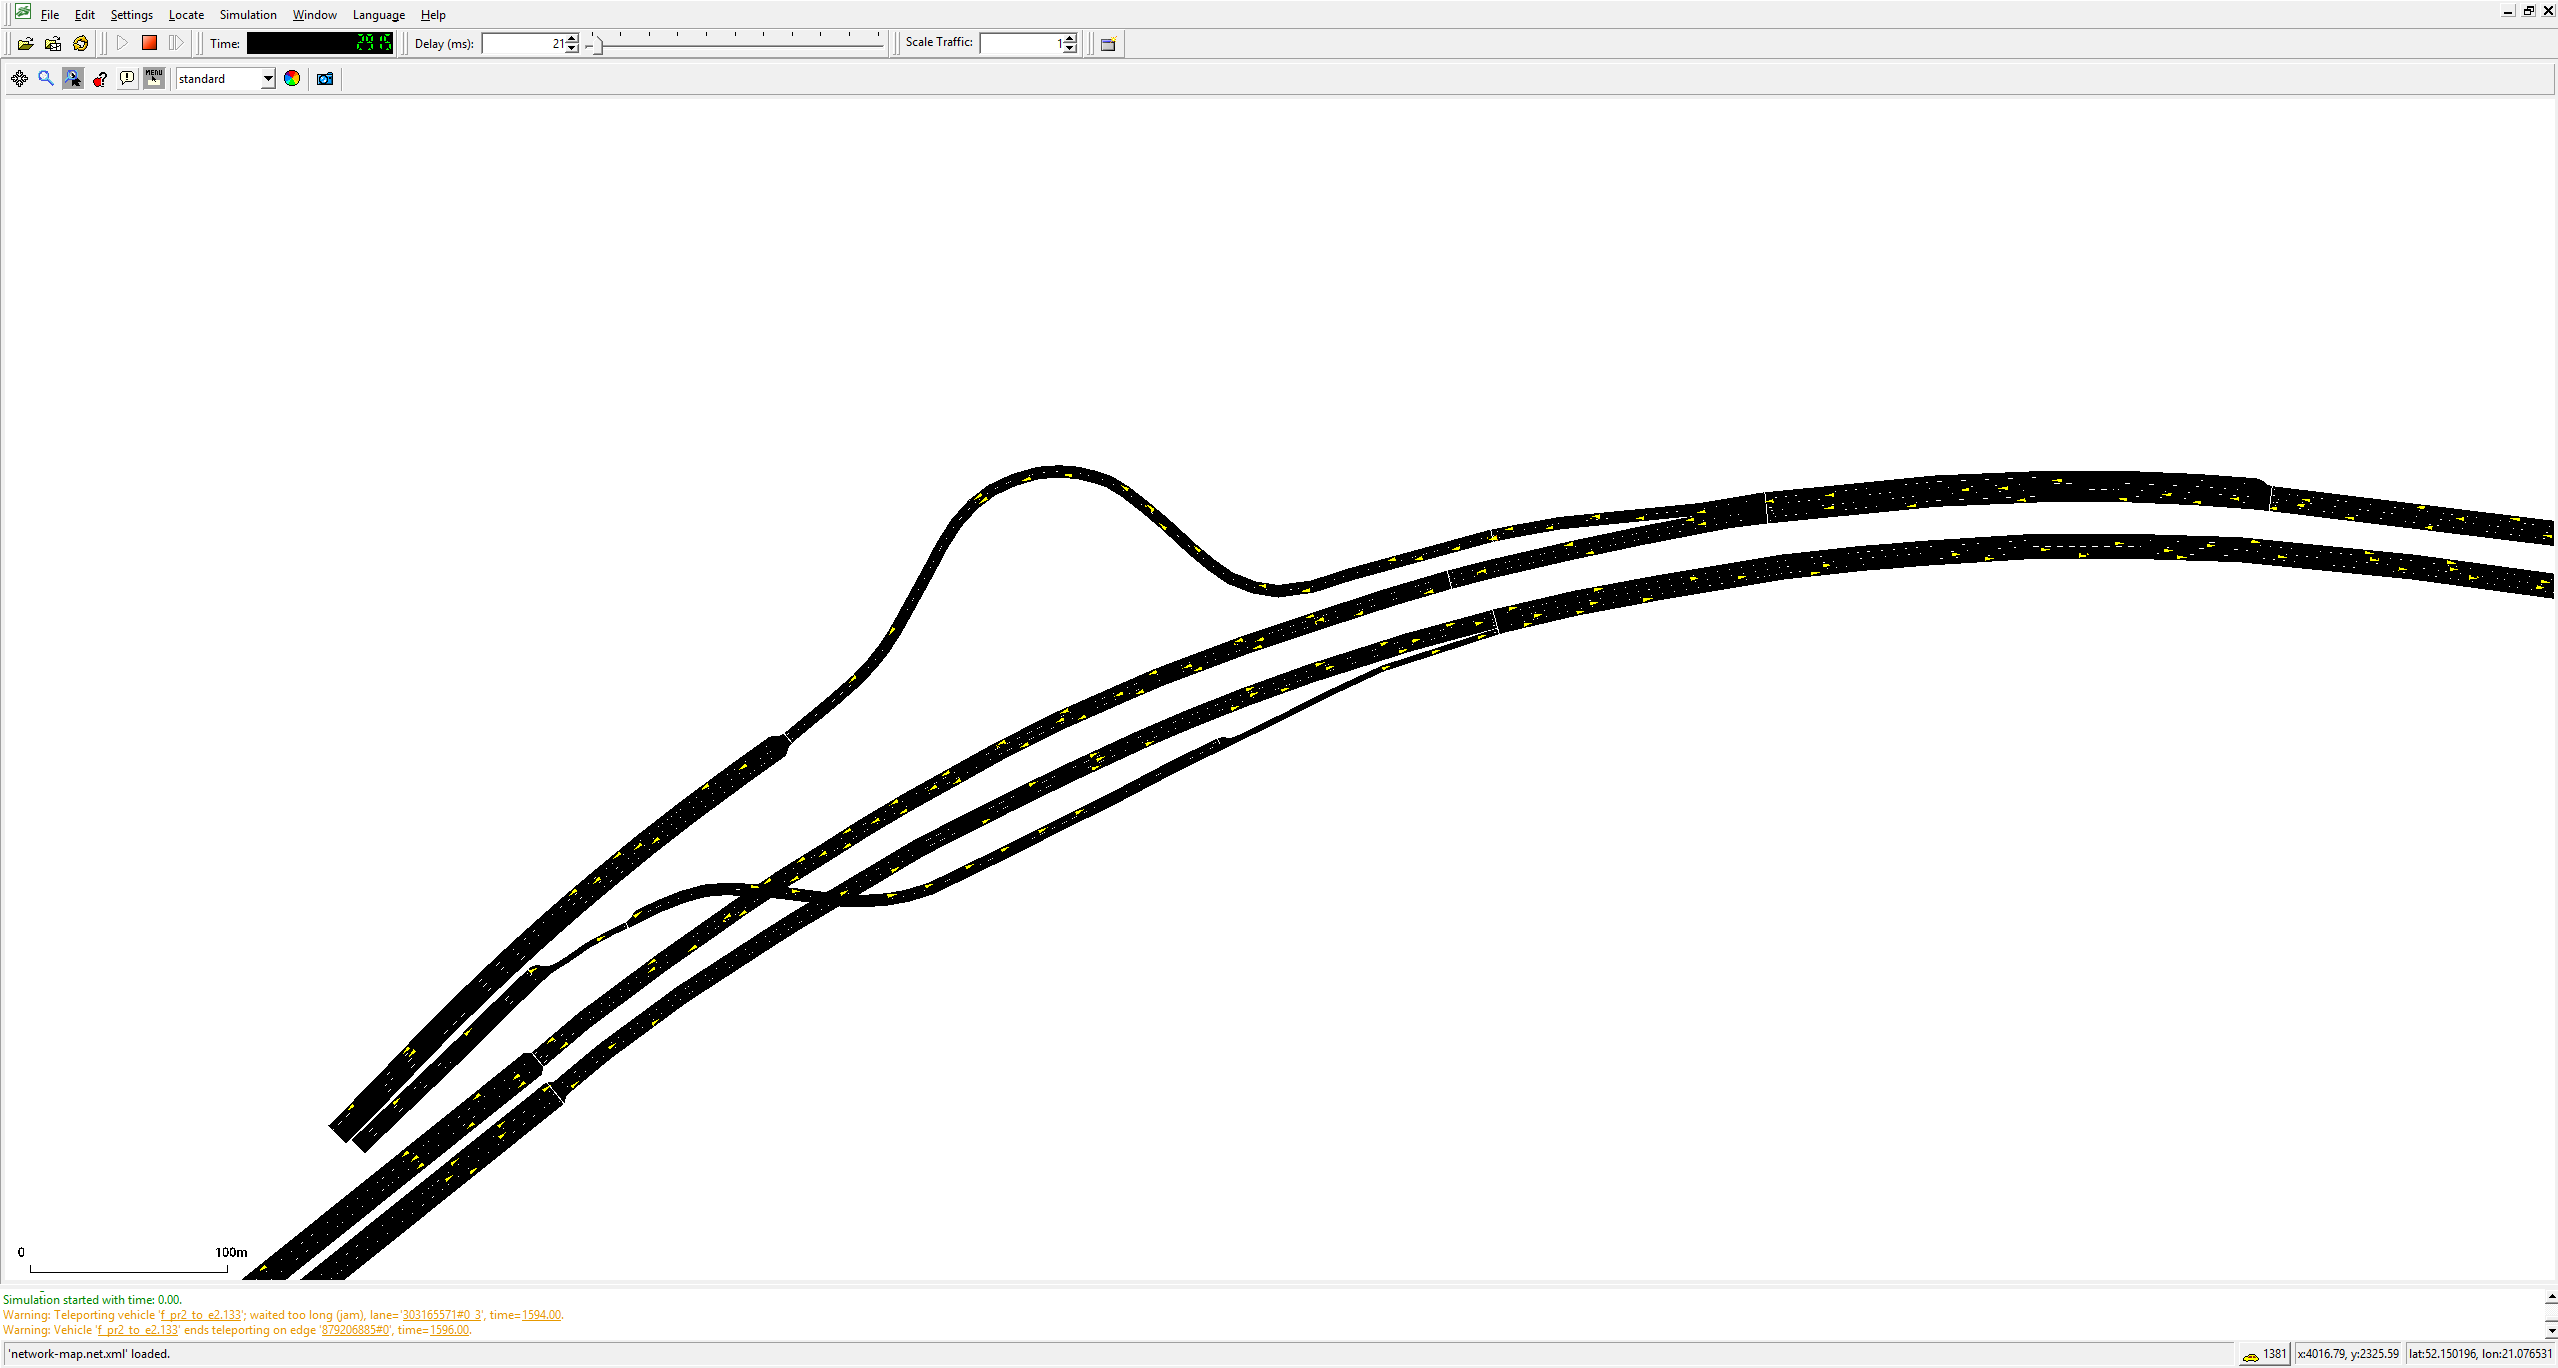
\includegraphics[width=0.9\linewidth]{img/simulation.png}
    \caption{Widok symulacji w interfejsie graficznym}
    \label{fig:simulation}
\end{figure}

%%%%%%%%%%%%%%%%%%%%%%%%%%%%%%%%%%%%%%%%%%%%%%%%%%%%%%%%%%%%%%%%%%%%%%%%%%%%%%%

\newpage

\section{Analiza symulacji dla różnych skali ruchu}

Przeprowadzenie symulacji było pierwszym celem projektu. Kolejnym celem jest próba zbadania przy pomocy wykorzystywanego symulatora płynności ruchu. \\

Narzędzie SUMO Eclipse udostępnia możliwość badania niektórych wartości, głównie uśrednionych, dotyczących symulacji. Wśród nich są m.in. prędkość ruchu oraz dane związane z czasem i opóźnieniem. Dane te możemy kolekcjonować poprzez systemowe wywołanie symulacji i dodanie odpowiednich flag na końcu wywołania: \\ 

\begin{itemize}
    \item \texttt{--duration-log.statistics},
    \item \texttt{--statistic-output}.
\end{itemize}

Dzięki takiemu wywołaniu symulacji autorzy zebrali dane z symulacji z pięciu różnych skal ruchu (Tabela~\ref{tab:statystyki_skalowania}). \\

\begin{table}[H]
\centering
\caption{Wpływ skalowania potoków ruchu na globalne parametry efektywności sieci}
\label{tab:statystyki_skalowania}

\setlength{\tabcolsep}{5.5pt} % Zwiększono z 3.5pt na 5.5pt, aby poszerzyć tabelę
\renewcommand{\arraystretch}{1.3}

\begin{tabular}{c|ccccccc}
\hline
\rotpion{Skala ruchu} & \multicolumn{1}{|c}{\rotatebox{90}{\rule{2mm}{0pt}\textbf{Pojazdy w symulacji}\rule{2mm}{0pt}}} & 
\rotpion{Śr. prędkość [m/s]} & 
\rotpion{Śr. czas podróży [s]} & 
\rotpion{Śr. czas oczekiwania [s]} & 
\rotpion{Śr. strata czasu [s]} & 
\rotpion{Śr. opóźnienie odjazdu [s]} & 
\rotpion{Liczba teleportacji} \\ \hline
0.5  & 9655  & 16.32 & 174.34 & 14.75  & 29.47  & 13.05   & 0  \\
0.75 & 14482 & 13.96 & 262.19 & 76.00  & 117.32 & 177.13  & 2  \\
1.0  & 19310 & 13.16 & 297.19 & 96.18  & 152.23 & 534.59  & 3  \\
1.2  & 23173 & 11.95 & 344.54 & 119.44 & 199.60 & 862.04  & 17 \\
1.4  & 27035 & 10.60 & 425.57 & 152.79 & 280.62 & 1251.92 & 38 \\ \hline
\end{tabular}
\end{table}

Wyniki symulacj potwierdzają wnioski oraz obserwacje analizy dotyczące tego, że wiele odcinków obwodnicy według prognoz na 2035r. będzie mocno obciążone. Wskazują na to średni czas oczekiwania. Na moment prognozy obwodnica w wielu miejscach będzie niewydolna (na co wskazywały w analizach oceny Poziomu Swobody Ruchu (PSR) na ocenę E lub D), jednak przyszłościowe zwiększenie ruchu będzie jeszcze bardziej wzmacniało ten efekt. 

%%%%%%%%%%%%%%%%%%%%%%%%%%%%%%%%%%%%%%%%%%%%%%%%%%%%%%%%%%%%%%%%%%%%%%%%%%%%%%%
\newpage

\section{Wnioski}

Przeprowadzona symulacja pozwoliła na odtworzenie prognozowanych warunków ruchu dla analizowanego fragmentu Południowej Obwodnicy Warszawy oraz ocenę zachowania infrastruktury przy zwiększonym natężeniu ruchu. Uzyskane wyniki wskazują, że przy prognozowanym ruchu na rok 2035 sieć drogowa będzie funkcjonowała blisko granicy swojej przepustowości, co znajduje odzwierciedlenie w wydłużonym czasie podróży, czasie oczekiwania oraz rosnących opóźnieniach pojazdów.\\

Analiza różnych skal ruchu wykazała wyraźną zależność pomiędzy natężeniem ruchu a efektywnością funkcjonowania infrastruktury. Wraz ze wzrostem liczby pojazdów następował spadek średniej prędkości przejazdu oraz wzrost wszystkich analizowanych wskaźników opóźnień. Szczególnie zauważalny był wzrost liczby teleportacji pojazdów w środowisku SUMO dla skal 1.2 i 1.4, co wskazuje na występowanie lokalnych zatorów oraz przekroczenie przepustowości wybranych elementów sieci. \\

Istotnym rezultatem projektu było również opracowanie własnej macierzy ruchu na podstawie danych zagregowanych dostępnych w dokumentacji inwestycji. Pomimo konieczności zastosowania pewnych uproszczeń i aproksymacji, uzyskane wartości charakteryzowały się niewielkimi odchyleniami od danych źródłowych, co pozwala uznać przygotowany model za wystarczająco wiarygodny do przeprowadzenia analiz porównawczych. \\

Wykorzystanie środowiska Eclipse SUMO okazało się odpowiednim wyborem do realizacji projektu. Narzędzie umożliwiło stosunkowo szybkie przygotowanie modelu infrastruktury, konfigurację ruchu oraz zebranie szczegółowych statystyk dotyczących funkcjonowania sieci drogowej. Dodatkową zaletą była możliwość wizualnej obserwacji ruchu oraz łatwego skalowania natężenia ruchu w celu przeprowadzania eksperymentów. \\

Otrzymane wyniki potwierdzają zasadność stosowania symulacji mikroskopowych jako narzędzia wspomagającego planowanie i ocenę inwestycji drogowych. Pozwalają one na identyfikację potencjalnych problemów związanych z przepustowością infrastruktury jeszcze przed ich wystąpieniem w rzeczywistych warunkach ruchu. \\

W przyszłości model mógłby zostać rozszerzony o dokładniejsze dane dotyczące struktury ruchu, uwzględnienie pojazdów ciężarowych, komunikacji zbiorowej oraz zmienności natężenia ruchu w zależności od pory dnia. Pozwoliłoby to na jeszcze dokładniejsze odwzorowanie rzeczywistych warunków eksploatacji analizowanego odcinka drogi. \\

%%%%%%%%%%%%%%%%%%%%%%%%%%%%%%%%%%%%%%%%%%%%%%%%%%%%%%%%%%%%%%%%%%%%%%%%%%%%%%%
\newpage
\printbibliography

%%%%%%%%%%%%%%%%%%%%%%%%%%%%%%%%%%%%%%%%%%%%%%%%%%%%%%%%%%%%%%%%%%%%%%%%%%%%%%%
\end{document}
